\begin{frame}
    \frametitle{Test Configuration (Config 1 Base)}
    \begin{itemize}
        \item Spatial domain size: 128 km \(\times\) 128 km \(\times\) 4 km \((x, y, z)\)
        \item Spatial grid: 0.25 km \(\times\) 0.25 km \(\times\) 0.125 km \((x, y, z)\)
        \begin{itemize}
            \item (this is the sea bottom mesh the parameter field is defined on, even if the FE code uses further refinement or high-order elements to resolve pressure and velocity)
        \end{itemize}
        \item Time domain: \((0, T)\); Simulation time \(T = 50\) s
        \item Temporal discretization of parameters and data: \(N_t = 500\) (10 Hz)
        \item ~132M (spatiotemporal) parameters and ~25K data points
        \item Quantity-of-interest (QOI): surface wave height in meters \((q)\)
        \item QOI temporal discretization: \(N_t^q = 50\) (1 Hz)
        \item Number of QOI spatial locations: \(N_q = 4 \(\times\) 4 = 16\)
    \end{itemize}
    \begin{figure}
        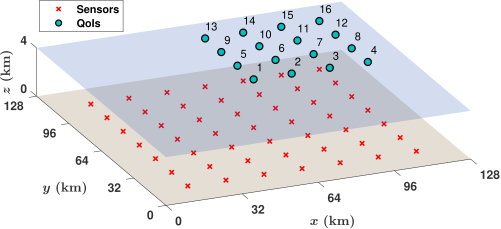
\includegraphics[width=0.5\textwidth]{JMM/images/test_config/sensor_qoi_locations.svg}
        \caption{Sensor and QOI Locations}
    \end{figure}
\end{frame}
